\section{Experiments for Proposal 1}\label{section:experiment_part_1}

{\color{red} TODO: short introduction}

\subsection{TF-IDF weighted Bag-of-words Features, Binary Relevance + Linear SVM Classifier}

{\color{red} TODO: short introduction, add one or two examples of people using this.}

\subsubsection{Results on Dataset 1}

\begin{figure}[H]
    \centering
    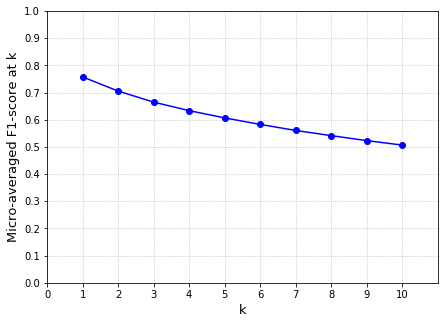
\includegraphics[width=7cm]{chapters/05_experiments/images/svm-tf-idf-delicious-20-frac.png}
    \caption{Results of applying Binary Relevance + Linear SVM with TF-IDF features on the Delicious t-140 Dataset (validation set scores shown)}
    \label{fig:ovr_svm_movielens}
\end{figure}

\subsubsection{Results on Dataset 2}

\begin{figure}[H]
    \centering
    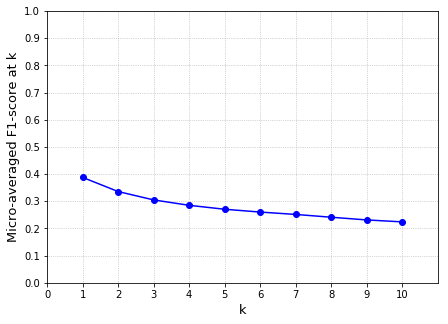
\includegraphics[width=7cm]{chapters/05_experiments/images/svm-tf-idf-movielens.png}
    \caption{Results of applying Binary Relevance + Linear SVM with TF-IDF features on the Movielens Dataset (validation set scores shown)}
    \label{fig:ovr_svm_movielens}
\end{figure}

\subsubsection{Discussion}

\begin{figure}[H]
    \centering
    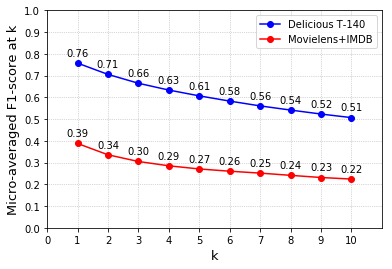
\includegraphics[width=7cm]{chapters/05_experiments/images/proposal-1-compared-ovr-svm-bow.png}
    \caption{Compared results (validation set scores)}
    \label{fig:compared_ovr_svm}
\end{figure}

As expected, the results in Dataset 1 were far better than those for Dataset 2, due to the differences in the tag distribution for both datasets.

It is interesting to note that the decrease in scores for Dataset 1 is somewhat more pronounced than in Dataset 2.

\subsection{TF-IDF weighted Bag-of-words Features, k-Nearest Neighbours Classifier}

The $k$-Nearest Neighbors is a very popular machine learning method that can be used both for classification and for regression. It consists in simply calculating the distances (assuming an $n$-dimensional representations) to every other instance, at \textit{inference time}\footnote{Methods such as $k$-NN are called \textit{lazy} methods because they need no training, as they defer all processing until actual inference is made.}. Then, each neighbor up to $k$ is treated as a source of information to help predict the class for the query instance. 

With respect to tag prediction, multiple (\cite{martinez_etal_2009,chidlovskii_2012,zhang_etal_2015,charte_etal_2015}\footnote{\cite{charte_etal_2015} have applied an approach very similar to ours, namely using multi-label $k$-NN to classify text into multiple tags, using TF-IDF representation. } to cite but a few) authors have applied some form of neighbor-based classifier to predicting tags for a query resource. 

In general, they proceed by finding nearest neighbors based on the resource's vector representation, as per the usual algorithm. Then, each neighbor's binary tag vector is added up and tags which are more commonly seen in the query instance's neighborhood are suggested.

Since we only want to use this method as a baseline, we implemented the most basic version thereof, namely simple, unweighted $k$-NN. Furthermore, we ran grid search over the method's hyperparameters, namely $k$, the number of neighbors to consider and also over the distance metric to use (cosine, euclidean, manhattan, etc).

\subsubsection{Results on dataset 1}

\begin{figure}[H]
    \centering
    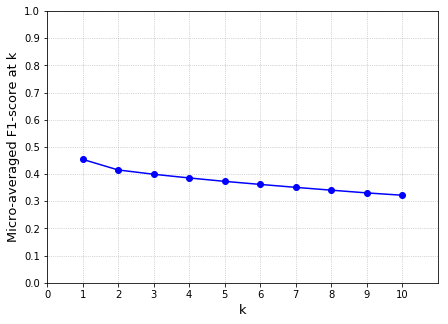
\includegraphics[width=7cm]{chapters/05_experiments/images/knn-tfidf-delicious.png}
    \caption{Applying $k$-NN on the Delicious Dataset, using TF-IDF weighted bag-of-words representation (validation set scores shown)}
    \label{fig:knn__movielens}
\end{figure}

\subsubsection{Results on Dataset 2}

\begin{figure}[H]
    \centering
    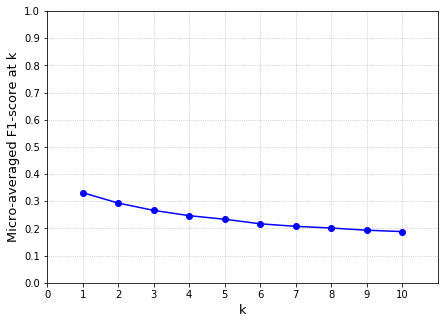
\includegraphics[width=7cm]{chapters/05_experiments/images/knn-tfidf-movielens.png}
    \caption{Applying $k$-NN on the Movielens Dataset, using TF-IDF weighted bag-of-words representation (validation set scores shown)}
    \label{fig:knn__movielens}
\end{figure}

\subsubsection{Discussion}

\begin{figure}[H]
    \centering
    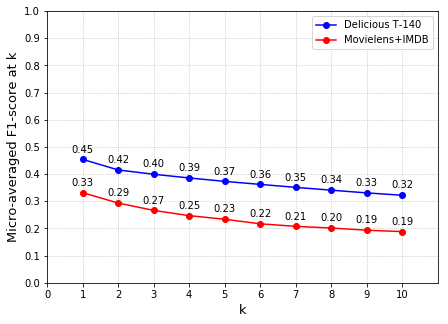
\includegraphics[width=7cm]{chapters/05_experiments/images/proposal-1-compared-knn-tfidf.png}
    \caption{Compared results (validation set scores)}
    \label{fig:compared_ovr_svm}
\end{figure}

Although the results were satisfactory, one can see that the difference in performance on both datasets is not as large as in the previous example. One reason for that may be that the large number of neighbours (found by model selection via grid search) may act as a regularizer, decreasing the variance on out-of-sample examples but at the cost of a higher bias.

 We would like to note that, surprisingly, using a \textit{weighted} variant did not increase performance on this task. In other words, weighing the contribution by the inverse of the distance to each neighbor did not increase the accuracy of the model.

\subsection{TF-IDF weighted Bag-of-words Features, Topic Distances}

In this approach, which has been suggested by \cite{choubey_2011},we first train a topic model on train set documents using Latent Dirichlet Allocation (LDA) (\cite{blei_etal_2003}). Then, at query time, we calculate the topic distribution for the query document and also the single most similar train set document, as measured by the Kullback-Leibler Divergence (KL-Divergence, \cite{kullback_leibler_1951}) between the topic distributions of the documents. Finally, the tags used in the found document are used as suggestions for the unlabelled query document.

\subsubsection{Results on dataset 1}

{\color{red} TODO}

\subsubsection{Results on Dataset 2}

\begin{figure}[H]
    \centering
    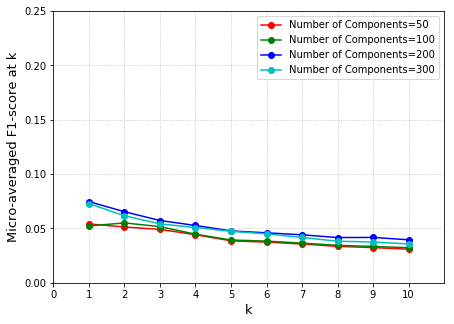
\includegraphics[width=7cm]{chapters/05_experiments/images/movielens-topic-distances.png}
    \caption{Applying Topic Distances on the Movielens Dataset, with varying values for the choice of LDA components}
    \label{fig:ovr_svm_movielens}
\end{figure}

\subsubsection{Discussion}

{\color{red} TODO mention results are around the same the original author got}

\subsection{TF-IDF weighted Bag-of-words Features, Topic Words}

In this approach, also suggested by \cite{choubey_2011}, one trains an LDA topic model on documents in the train set. At test time, the topic distribution for each query document is calculated with the trained model. Then, the most representative words \footnote{Only words that are in the actual tag vocabulary are used.} for the most representative topic are suggested as tags for the query document.

\subsubsection{Results on dataset 1}

{\color{red} TODO}

\subsubsection{Results on Dataset 2}

\begin{figure}[H]
    \centering
    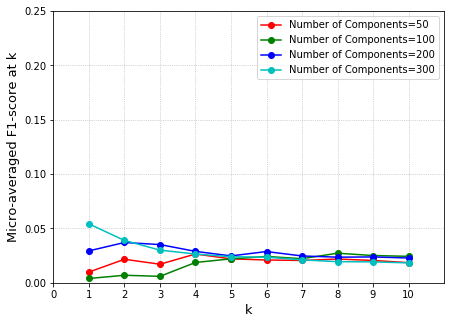
\includegraphics[width=7cm]{chapters/05_experiments/images/movielens-topic-words.png}
    \caption{Applying Topic Words on the Movielens Dataset, with varying values for the choice of LDA components}
    \label{fig:ovr_svm_movielens}
\end{figure}

\subsubsection{Discussion}

{\color{red} TODO mention results are around the same the original author got}

\subsection{LDA Topic Probabilities, k-nearest Neighbours Classifier}\label{sub:lda_topics}

Although Latent Dirichlet Allocation (LDA) \citep{blei_etal_2003} was originally created as a means to infer representative words for topics in corpora, it can be (and frequently is) used to extract features for documents. In fact, this approach was used and suggested in the original paper itself.

In other words, LDA can be used as a form of dimensionality reduction to reduce the size of feature vectors\footnote{Assuming an original bag-of-words representation without trimming the number of words used.} from $V$ to $k$, respectively the vocabulary size and the number of components in the LDA model.

Using these topic probabilities as features, we can then proceed onto classifying the documents using any classifier we wish. We have chose to use two classifier for this task: \textbf{a)} a simple $k$-nearest Neighours Classifier so as to enable comparison between using LDA features and using bag-of-words features and \textbf{b)} (in the next subsection) an SVM classifier, as suggested in the original LDA article.

\subsubsection{Results on dataset 1}

{\color{red} TODO}

\subsubsection{Results on Dataset 2}

\begin{figure}[H]
    \centering
    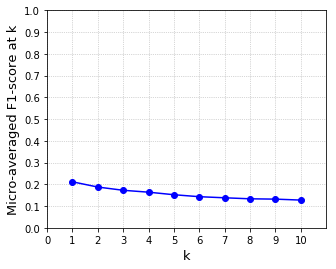
\includegraphics[width=7cm]{chapters/05_experiments/images/knn-lda-movielens.png}
    \caption{k-Nearest Neighbor classifier on the Movielens dataset, using LDA topic probabilities as features.}
    \label{fig:knn_lda_movielens}
\end{figure}

\subsubsection{Discussion}

\subsection{LDA Topic Probabilities, SVM classifier}

As mentioned on the previous subsection, we will compare results between both datasets using LDA as a simple dimensionality reduction step on top of TF-IDF weighted bag-of-words features. We will use an SVM classifier, as suggested in the original LDA paper by \cite{blei_etal_2003}.

\subsubsection{Results on dataset 1}

{\color{red} TODO}

\subsubsection{Results on Dataset 2}

\begin{figure}[H]
    \centering
    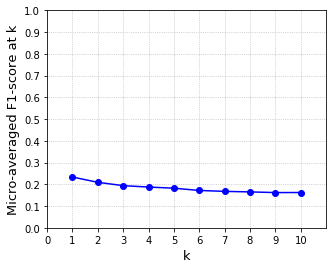
\includegraphics[width=7cm]{chapters/05_experiments/images/svm-lda-tf-idf-movielens.png}
    \caption{SVM classifier on the Movielens dataset, using LDA topic probabilities as features.}
    \label{fig:svm_lda_movielens}
\end{figure}

\subsubsection{Discussion}

{\color{red} TODO}

\subsection{Final Results and discussion}

{\color{red} TODO: as expected, results in dataset 1 were better but some were better, maybe because it's the way the features are represented.}

{\color{red} TODO: maybe it's because documents  in dataset 1 represent the resource itself (a webpage) while in dataset 2 the documents are a *description* of the resource, not the resource itself (resources are movies). In a way it's secondhand information.}

{\color{red} TODO: plot all experiments on a single graph to help people compare them}
